%\documentclass[german,10pt]{book}      
\usepackage{makeidx}
\usepackage{babel}            % Sprachunterstuetzung
\usepackage{amsmath}          % AMS "Grundpaket"
\usepackage{amssymb,amsfonts,amsthm,amscd} 
\usepackage{mathrsfs}
\usepackage{rotating}
\usepackage{sidecap}
\usepackage{graphicx}
\usepackage{color}
\usepackage{fancybox}
\usepackage{tikz}
\usetikzlibrary{arrows,snakes,backgrounds}
\usepackage{hyperref}
\hypersetup{colorlinks=true,
                    linkcolor=blue,
                    filecolor=magenta,
                    urlcolor=cyan,
                    pdftitle={Overleaf Example},
                    pdfpagemode=FullScreen,}
%\newcommand{\hyperref}[1]{\ref{#1}}
%
\definecolor{Gray}{gray}{0.80}
\DeclareMathSymbol{,}{\mathord}{letters}{"3B}
%
\newcounter{num}
\renewcommand{\thenum}{\arabic{num}}
\newenvironment{anmerkungen}
   {\begin{list}{(\thenum)}{%
   \usecounter{num}%
   \leftmargin0pt
   \itemindent5pt
   \topsep0pt
   \labelwidth0pt}%
   }{\end{list}}
%
\renewcommand{\arraystretch}{1.15}                % in Formeln und Tabellen   
\renewcommand{\baselinestretch}{1.15}                 % 1.15 facher
                                                      % Zeilenabst.
\newcommand{\Anmerkung}[1]{{\begin{footnotesize}#1 \end{footnotesize}}\\[0.2cm]}
\newcommand{\comment}[1]{}
\setlength{\parindent}{0em}           % Nicht einruecken am Anfang der Zeile 

\setlength{\textwidth}{15.4cm}
\setlength{\textheight}{23.0cm}
\setlength{\oddsidemargin}{1.0mm} 
\setlength{\evensidemargin}{-6.5mm}
\setlength{\topmargin}{-10mm} 
\setlength{\headheight}{0mm}
\newcommand{\identity}{{\bf 1}}
%
\newcommand{\vs}{\vspace{0.3cm}}
\newcommand{\noi}{\noindent}
\newcommand{\leer}{}

\newcommand{\engl}[1]{[\textit{#1}]}
\parindent 1.2cm
\sloppy

         \begin{document}  \setcounter{chapter}{4}

\chapter{Zeitmessung}
% Kap 5
\label{chap_Uhren}


\info{Thomas Filk}{28.03.2024}%
Im Jahre 1967 wurde beschlossen, die Sekunde \"uber den Hyperfeinstruktur\"ubergang
von 133-C\"asium im Grundzustand zu definieren: Eine Sekunde entspricht der Zeitdauer von
9\,192\,631\,770 Schwingungen zu diesem \"Ubergang.\index{Sekunde} 
Damit erhebt sich die Frage, wie man die Zeit
\"uberhaupt messen kann. Die Geschichte der Zeitmessung ist eines der spannendsten Kapitel
in der Geschichte der Physik. 

\section{Antike Zeitmesser}

F\"ur gro\ss e Zeitr\"aume dienten in der Antike immer die nat\"urlichen
Einheiten Tag und Monat, die sich leicht aus der Bewegung der Sonne (bzw.\ der Drehung der Erde) 
und des Monds bestimmen lie\ss en.
Auch wenn der Zyklus eines Jahres etwas schwieriger festzustellen war, kannte
man schon in den fr\"uhen Kulturen Verfahren, mit deren Hilfe man beispielsweise die Tag-und-Nacht-Gleiche
oder die Sommersonnenwende und damit ein Kalendersystem festlegen konnte. 
Schon den Babyloniern war bekannt, dass die vier astronomischen Jahreszeiten - die Zeiten
zwischen den Tag-und-Nacht-Gleichen (Fr\"uhling und Herbst) und den Sonnenwenden
(Sommer und Winter) - nicht gleich lang waren. Heute wissen wir, dass dies an der
elliptischen Umlaufbahn der Erde um die Sonne liegt: Beim sonnenn\"achsten Punkt der Erdbahn
(dem Perihel - derzeit zwischen dem 2.\ und 5.\ Januar) bewegt sich die Erde nach dem zweiten Kepler'schen
Gesetz etwas schneller um die Sonne als beim sonnen\-fernsten Punkt, dem Aphel (derzeit um den 3.-6.\ Juli).  
Und Ptolem\"aus wusste ebenfalls, dass sich die Sonne gleichm\"a\ss ig entlang der Ekliptik bewegt und somit
nicht gleichm\"a\ss ig entlang der Projektion der Sonnenbahn auf den \"Aquator 
bzw.\ die L\"angengrade \cite{Neugebauer}. Die Korrekturen zwischen
wahrem und mittlerem Sonnentag - die Zeitgleichung - werden schon bei Ptolem\"aus beschrieben, auch wenn
sie erst im 17.\ Jahrhundert mit den Kepler'schen Gesetzen erkl\"art werden konnten.
Im Folgenden geht es jedoch eher um die Einteilung des Tages in Untereinheiten und die Messung
von kurzen Zeitr\"aumen.

\subsection{Sonnenuhren}

Ein wichtiges und nat\"urliches Zeitma\ss\ war seit jeher die Sonnenuhr.\index{Sonnenuhr} 
Schon in vorhistorischen Zeiten d\"urften die Schatten von Felsvorspr\"ungen, B\"aumen oder Str\"auchern
und \"ahnlichen nat\"urlichen Gegenst\"anden beobachtet und dadurch eine
Tageseinteilung vorgenommen worden sein. Man wird auch fr\"uh festgestellt haben, dass
die Sonne zu verschiedenen Jahreszeiten eine unterschiedliche H\"ohe hat und somit
die Schattenl\"ange an einer Sonnenuhr von der Jahreszeit abh\"angt. 

An manchen Sonnenuhren wurde diese jahreszeitliche Abh\"angigkeit genutzt, um die angezeigte
wahre Sonnenzeit \"uber ein sogenanntes Analemma (eine Figur in Form einer verzerrten Acht, mit
der die Zeitgleichung so auf die Uhr projiziert wird, dass man aus dem Schatten die mittlere
Sonnenzeit ablesen kann)\index{Analemma} 
mit der mittleren Sonnenzeit in Bezug zu setzen (siehe Abb.\ \ref{fig_Munich_Analemma}).

\begin{figure}[htb]
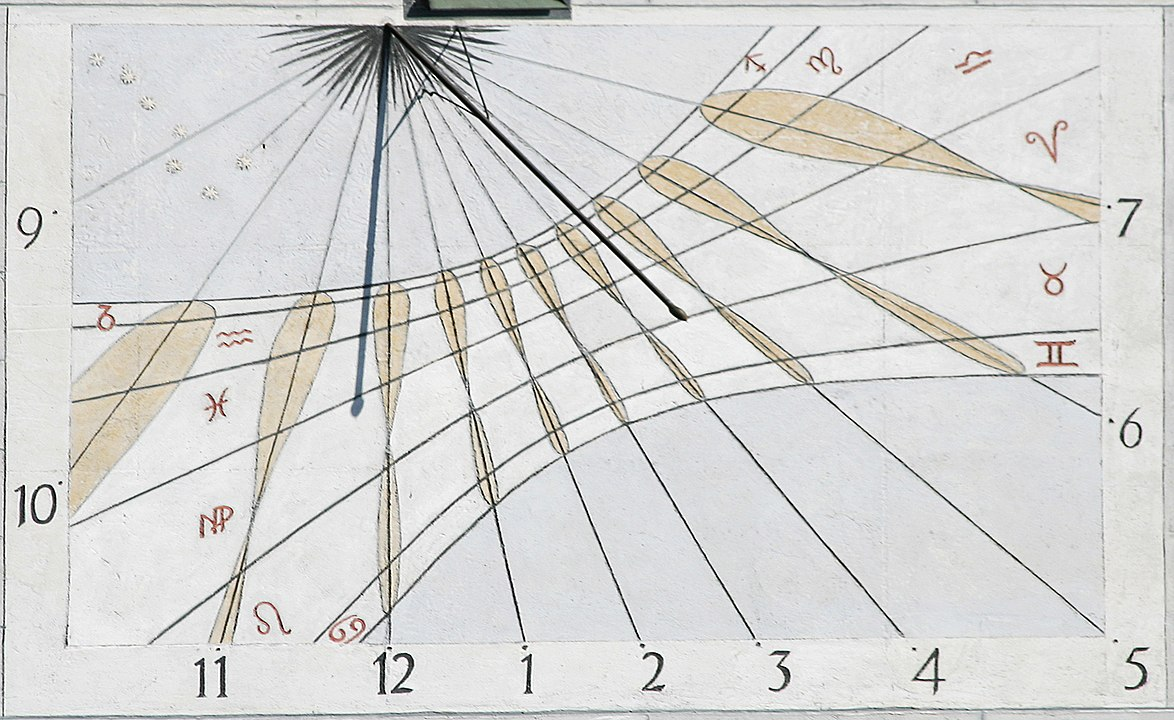
\includegraphics[width=0.8\textwidth]{./Bilder/Munich_Altes_Rathaus_sundial.jpg}
\caption{\label{fig_Munich_Analemma}%
Sonnenuhr am Alten Rathaus in M\"unchen. Anhand der Schattenl\"ange zu verschiedenen Jahreszeiten
kann die wahre (angezeigte) Uhrzeit um die Zeitgleichung korrigiert werden, die durch die
Analemmas an den Stundenlinien angegeben wird. Die Sternzeichen geben an, welcher
Teil des Analemmas (linker oder rechter Rand) in einem bestimmten Monat zu verwenden ist. (aus \cite{Niermann})} 
\end{figure}

Das Analemma ist gleichzeitig ein Bild der Sonnenst\"ande am Himmel: Macht man t\"aglich
zur selben mittleren Uhrzeit ein Bild vom Sonnenstand, so ergibt sich im Verlauf eines Jahres die Form
des Analemmas.  

\subsection{Wasseruhren und andere Zeitmesser des Altertums}

Ein Hilfsmittel zur Reproduktion gleicher Zeitr\"aume war auch die Klepshydra: 
ein mit Wasser\index{Klepshydra}\index{Wasseruhr}
gef\"ulltes Gef\"a\ss\ mit einer kleinen \"Offnung an der unteren Seitenwand oder im Boden, 
durch die das Wasser auslaufen
konnte, das dann in einem zweiten Gef\"a\ss\ aufgefangen wurde. Mit solchen Klepshydren wurden
beispielsweise die Redezeiten bei politischen Versammlungen oder auch bei Gerichtsprozessen im alten 
Griechenland und Rom
gemessen. Vermutlich geht hierauf der Begriff \glqq seine Zeit ist abgelaufen\grqq\ zur\"uck. Noch heute
beruht die Sanduhr, gelegentlich zum Eierkochen oder auch bei Gesellschaftspielen verwendet, 
auf diesem Prinzip.

Im fr\"uhen Mittelalter wurden die Klepshydren zu komplizierteren Wasseruhren abgewandelt. 
Dabei handelte es sich um teilweise sehr aufwendige Anlagen, durch die Wasser aus einem
oberen Reservoir in ein tiefer gelegenes Reservoir floss und dabei komplexe Mechanismen
in Gang setzte. Manche dieser Mechanismen glichen auch schon den sp\"ateren Hemmungen.

Insbesondere in Kl\"ostern, wo teilweise auch zu Nachtstunden zum Gebet aufgerufen wurde, kamen sp\"ater
sogenannte\index{Stundenkerze} 
Stundenkerzen - Kerzen genormter Dicke, bei denen Markierungen den groben
Stundenverlauf anzeigten - hinzu. Einem \"ahnlichen Zweck dienten auch \"Olkerzen, bei denen
ein Docht in ein mit \"Ol gef\"ulltes Gef\"a\ss\ ragte und am anderen Ende brannte. Die
verflossene Zeit konnte an dem verbrauchten \"Ol abgelesen werden.

\section{Uhren}

Um 1300 erlaubte die Erfindung der sogenannten Hemmung die Konstruktion der
ersten R\"aderuhren und damit von mechanischen Uhren, die auf oszillatorischen Prozessen beruhen. 
Wer den Mechanismus der Hemmung erfunden hat oder wann genau dieser
Mechanismus erfunden wurde, ist nicht bekannt. Wir wissen heute lediglich, dass um 1300 die
ersten Uhren entstanden sind, die auf diesem Prinzip beruhen. 

\subsection{Hemmungen}

Eine Hemmung\index{Hemmung} 
erlaubt es, eine mechanische Kraft (z.B.\ eine Gewichtskraft) in eine regelm\"a\ss ige Bewegung
umzuwandeln. H\"angt beispielsweise ein Gewicht an einem langen Seil, aufgewickelt auf eine
frei drehbare Rolle, so w\"urde ungehemmt das Gewicht mit wachsender Geschwindigkeit
absinken und die Rolle w\"urde sich mit zunehmender Geschwindigkeit drehen. Eine Hemmung
bewirkt, dass diese Drehung in eine meist abgehackte, konstant periodische Bewegung umgewandelt wird
und somit f\"ur eine Zeitmessung verwendet werden kann. Die \"altesten Hemmungen sind die
sogenannten Spindelhemmungen\index{Spindelhemmung}\index{Foliot} 
mit einem Foliot -- einem hin und her schwingenden Querbalken mit Gewichten, 
der \"uber eine vertikale Achse mit zwei Pl\"attchen in ein Zahnrad\index{Kronrad} 
(das Kronrad) eingreift (siehe Abb.\ \ref{fig_Foliot}) -- oder\index{Unrast}
einer Unrast, einer rotierende Scheibe, die ansonsten nach einem 
\"ahnlichen Mechanismus wie das Foliot arbeitet.

\begin{figure}[htb]
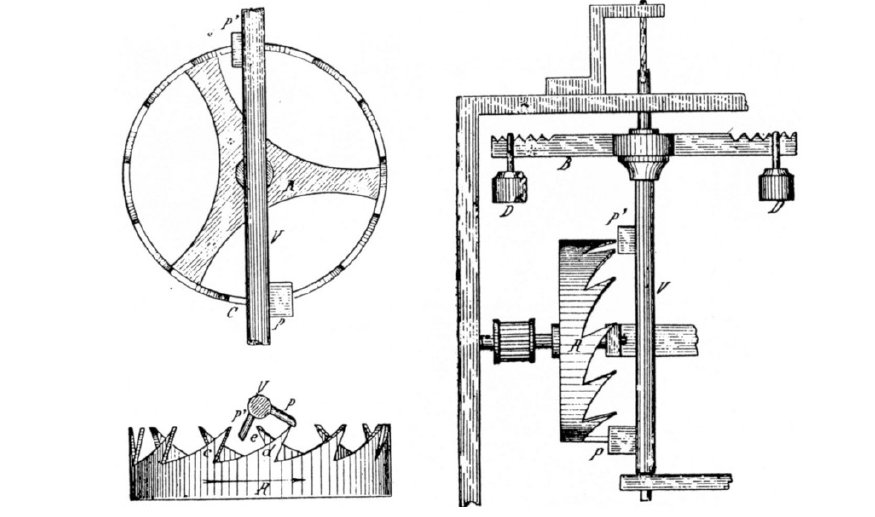
\includegraphics[width=0.7\textwidth]{./Bilder/Foliot.jpg}
\caption{\label{fig_Foliot}%
Eine Spindelhemmung mit Foliot. Das Kronrad $R$ wird \"uber ein Gewicht, das an einem \"uber die
Achse des Kronrads gewickelten Seil h\"angt (nicht dargestellt), angetrieben. Das Foliot $B$ mit den Gewichten $D$
besteht aus einem waagerechten Balken, der fest mit einer vertikalen Achse $V$ verbunden ist. 
An dieser Achse befinden sich zwei Pl\"attchen $P$ und $P'$, die abwechselnd oben und unten in die
Z\"ahne ($c$, $d$ und $e$) des Kronrads $R$ einhaken. 
Dies f\"uhrt zu einer Hin- und Herbewegung des Foliots und damit
zu einer kontrollierten, langsamen, abgehackt gleichm\"a\ss igen Drehung des Kronrads. \"Uber die Gewichte kann
die Schwingungsfrequenz des Foliots und damit der Gang der Uhr reguliert werden.
(aus \cite{Foliot})}
\end{figure}
 
 Ein Video mit dem Mechanismus einer Spindelhemmung findet man unter \cite{Verge}. 
 \"Uber Zahnradmechanismen, die im Mittelalter schon lange bekannt waren, 
 kann die Drehung des Kronrads auf andere R\"ader \"ubertragen und
 dabei beliebig verlangsamt werden. Bis zum 17.\ Jahrhundert erreichten Uhren mit Spindelhemmungen eine
 Genauigkeit von rund 15 Minuten pro Tag. 
 
 \subsection{Pendeluhren}

Im 17.\ Jahrhundert wurde die Spindelhemmung durch die mit einem Pendel gekoppelte 
Ankerhemmung\index{Ankerhemmung}\index{Pendeluhr}
ersetzt (siehe Abb.\ \ref{fig_Anker}). 
Nachdem Galileo\index{Galilei, Galileo} 
um 1630 festgestellt hatte, dass die Periode eines Pendels f\"ur kleine Auslenkungen 
nahezu unabh\"angig von dieser Auslenkung ist, erkannte man, dass sich das Pendel im Vergleich zum Foliot 
besser als Taktgeber eignet. Durch das Drehmoment, das \"uber ein Gewicht auf das Kronrad \"ubertragen
wird, gibt das Kronrad bei seinem Weiterdrehen \"uber den Anker umgekehrt dem Pendel regelm\"a\ss ig 
einen kleinen Sto\ss, sodass dieses 
mit einer kleinen aber konstanten Auslenkung schwingt und nicht durch Reibungseffekte zur Ruhe kommt. 

\begin{figure}[htb]
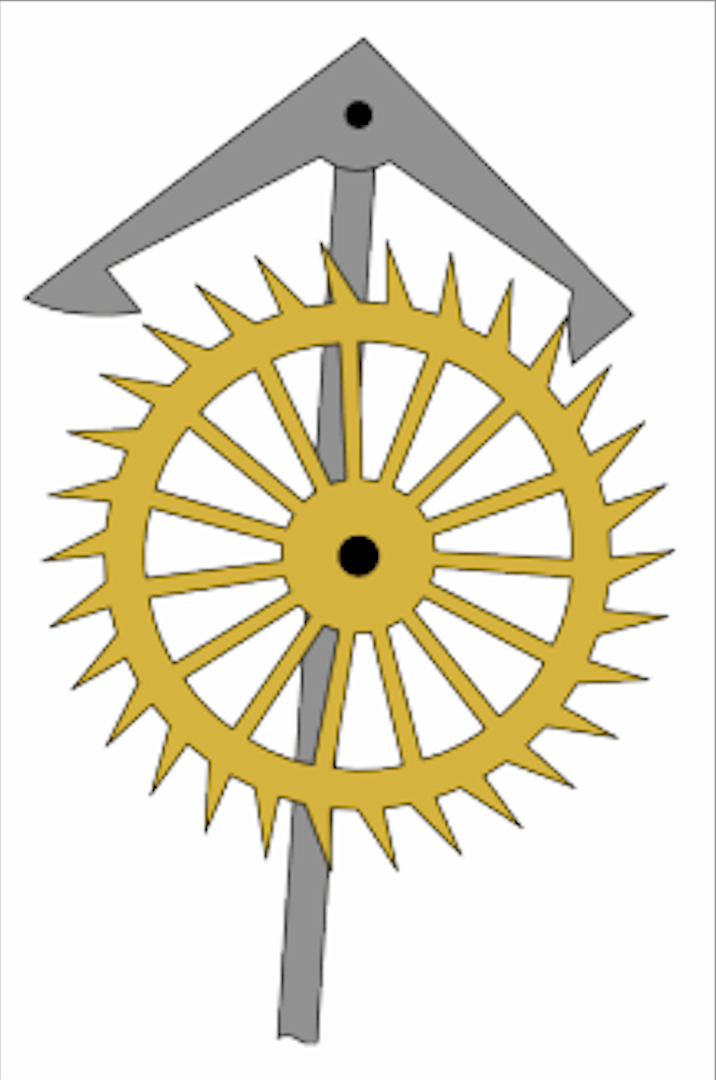
\includegraphics[trim=2 2 2 2,clip,width=0.245\textwidth]{./Bilder/Anker_10.png}
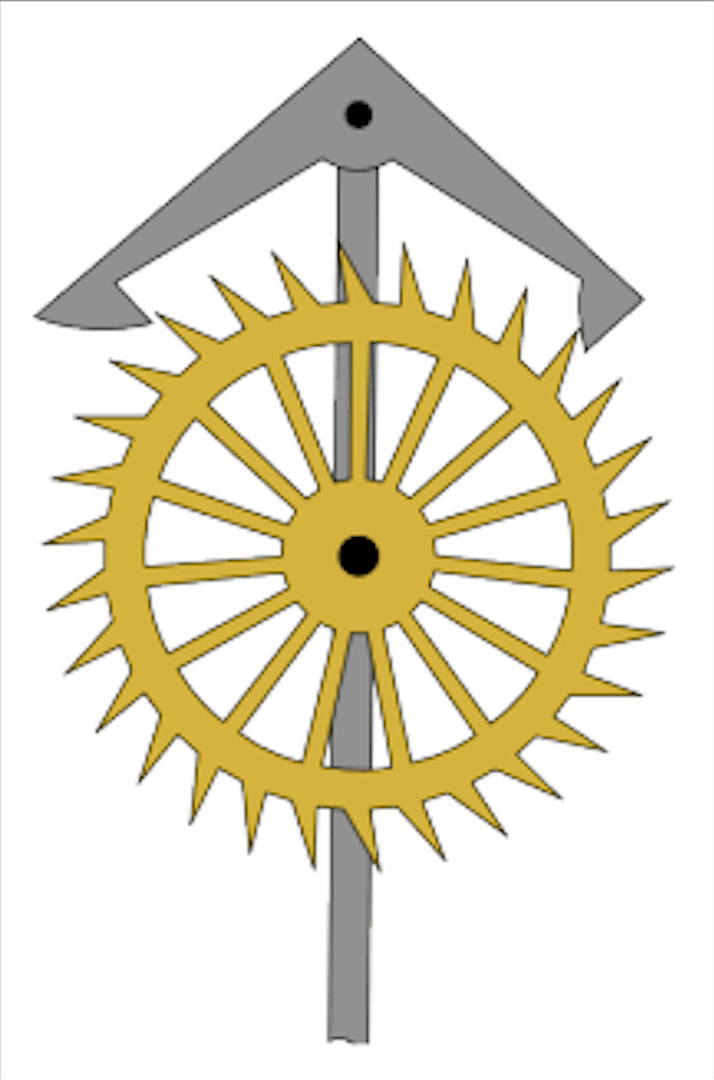
\includegraphics[trim=2 2 2 2,clip,width=0.245\textwidth]{./Bilder/Anker_18.png}
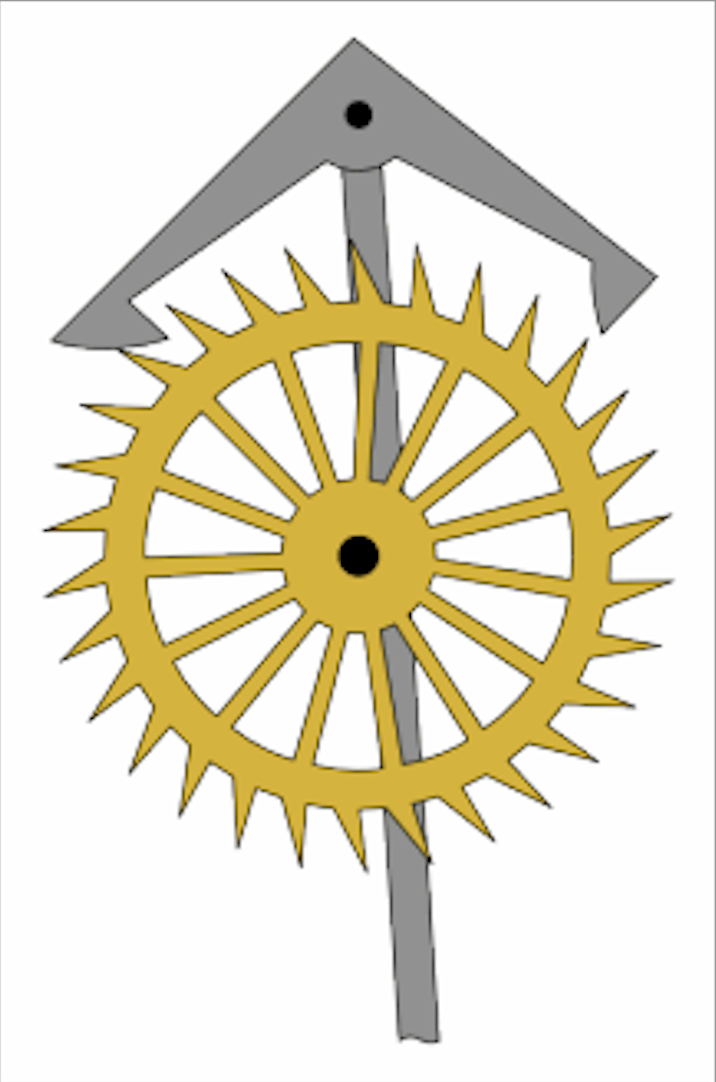
\includegraphics[trim=2 2 2 2,clip,width=0.245\textwidth]{./Bilder/Anker_27.png}
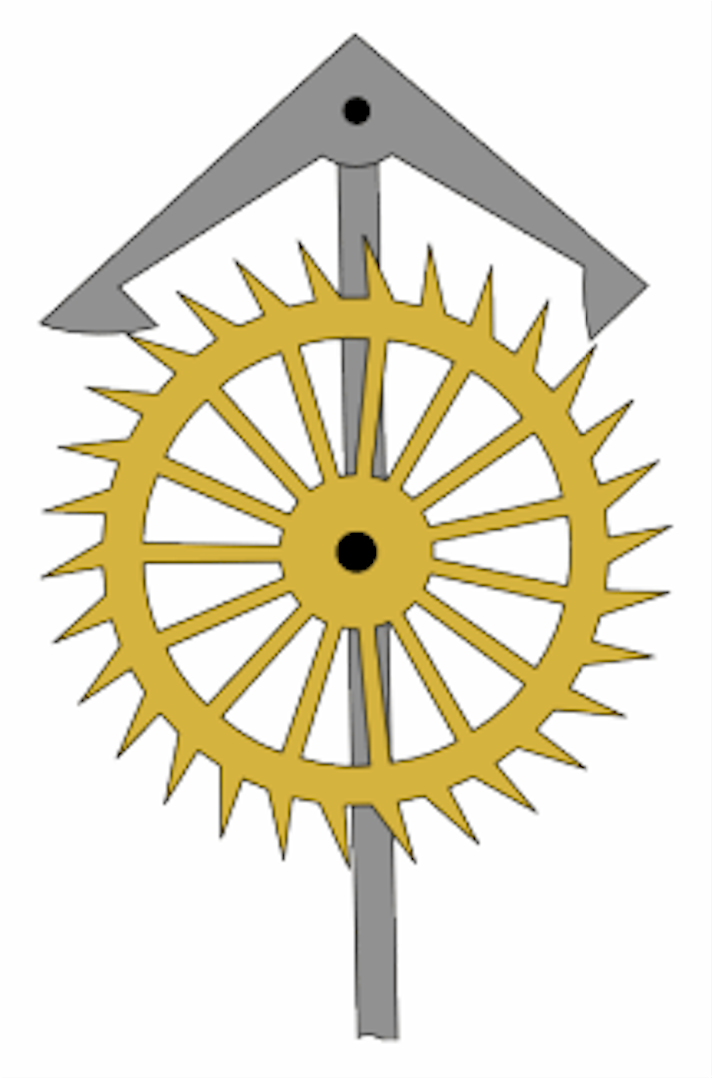
\includegraphics[trim=2 2 2 2,clip,width=0.245\textwidth]{./Bilder/Anker_35.png}
\caption{\label{fig_Anker}%
Eine Ankerhemmung. Der Anker ist fest mit einem Pendel verbunden und wenn das Pendel schwingt, greift
der Anker abwechselnd rechts und links in die Zacken des Kronrads. Das Kronrad dreht sich im Uhrzeigersinn
und wird von einem Gewicht (nicht dargestellt) angetrieben. Bei jeder Vorw\"artsbewegung \"ubertr\"agt es 
aufgrund der Zackenform und der Form des Ankerhakens einen kleinen Sto\ss\ auf den Anker und damit auf
das Pendel. (aus \cite{Verge})}
\end{figure}

Christiaan Huygens\index{Huygens, Christiaan}\index{Hooke, Robert} 
entwickelte um 1656 eine Uhr auf dem Prinzip der Pendeluhr. Nachdem Robert Hooke
1658 die Ankerhemmung erfunden hatte, die eine kleine Schwingungsauslenkung des Pendels erm\"oglichte und damit
eine h\"ohere Genauigkeit in der Pendelperiode, wurde die Pendeluhr zum Standard in der Uhrenkonstruktion. 
Hier zeigt sich das Grundprinzip der heutigen Uhren: Eine harmonische Schwingung dient einerseits
als Standard f\"ur die Zeitmessung, andererseits wird sie durch den Mechanismus der R\"uckkopplung
von einer \"au\ss eren Kraft (hier das Gewicht, welches das Kronrad antreibt) aufrecht erhalten. 

\section{Das Problem des L\"angengrads}

Die Eroberung Konstantinopels\index{Konstantinopel} 
im Jahre 1453 durch die osmanischen Truppen markiert einen
entscheidenden Wendepunkt in der Geschichte des Abendlands. Oftmals wird in diesem Ereignis eine 
Ursache f\"ur den Wechsel vom Mittelalter zur Neuzeit gesehen. Diese Eroberung nach einer
langen Belagerung l\"oste zwei Bewegungen aus:
(1) Nachdem der Landweg von Europa zu den attraktiven Handelspl\"atzen in Indien, 
Indonesien und China im Wesentlichen gesperrt bzw.\ unter islamischer Kontrolle war, was oft
hohe Abgaben bzw.\ Z\"olle zur Folge hatte,
suchte man nach anderen Wegen nach Indien. Dies f\"uhrte nicht nur zur Umsegelung Afrikas,
sondern auf der Suche nach einem direkten Weg nach Indien auch zur Entdeckung Amerikas und
des Pazifischen Ozeans. (2) Die Flucht vieler Gelehrter aus Konstantinopel in den Westen,
die in ihrem Gep\"ack oft wertvolle B\"ucher mit sich f\"uhrten, l\"oste die\index{Renaissance}
Renaissance aus -- auf diese Weise wurden viele antike Schriften, teilweise in ihren
arabischen \"Ubersetzungen, im Westen erst bekannt.  

Insbesondere die Erkundungsfahrten zur See brachten einige Probleme auf: Bis zu Beginn
des 15.\ Jahrhunderts beschr\"ankten sich Seefahrten haupts\"achlich auf den Mittelmeerraum
oder aber auf Fahrten entlang der europ\"aischen K\"usten nach Norden (Frankreich, England, 
Norwegen) oder entlang der afrikanischen K\"uste nach S\"uden (bei dieser Gelegenheit wurden
die Kanarischen Inseln sowie sp\"ater die Inselgruppe um Madeira und die Azoren entdeckt). Im Verlauf
des 15.\ Jahrhunderts erkundete man haupts\"achlich den Seeweg um Afrika nach Indien, der
dann von Vasco da Gama\index{Vasco da Gama} 
im Jahre 1498 auch gefunden wurde und eine Route von
Europa nach Indien und China er\"offnete, die nicht durch islamisch
kontrolliertes Gebiet f\"uhrte. Eine solche Umsegelung Afrikas war
m\"oglich, ohne \"uber einen l\"angeren Zeitraum hinweg die K\"uste als Anhaltspunkt f\"ur die
Ortsbestimmung aus dem Blickfeld zu verlieren. Allerdings war diese Schiffsroute sehr lang
und wegen der vielen Piraten in der N\"ahe des Horns von Afrika auch recht gef\"ahrlich.

Die andere M\"oglichkeit sah man in einer direkten Route von Europa nach Indien auf einem Weg
in Richtung Westen.\index{Columbus, Christoph} 
Diesen Weg wollte Columbus finden und entdeckte auf diese Weise
1492 das heutige Amerika (genauer entdeckte er eine Insel der Bahamas). W\"ahrend eine Umfahrung Afrikas
noch mit visuellem K\"ustenkontakt m\"oglich war, musste man f\"ur die Westroute die
vertrauten K\"usten Europas und Afrikas verlassen. Nachdem Columbus die Bahamas entdeckt hatte 
und in der Folgezeit auch L\"ander auf dem amerikanischen Festland
(sowohl in Nord- als auch S\"udamerika) entdeckt wurden, und nachdem 
Ferdinand Magellan\index{Magellan, Ferdinand} 
um 1520 die erste Umsegelung S\"udamerikas und die \"Uberquerung des Pazifischen Ozeans
gelang, wurde das Problem der genauen Ortsbestimmung der neu entdeckten L\"ander und
Inseln wichtig. Zum Einen wollten die Herrscher, die solche Erkundungsfahrten der Seefahrer
finanzierten und die dabei entdeckten L\"ander f\"ur sich in Anspruch nahmen, wissen, wo 
genau sich diese L\"ander befanden, d.h.\ es kam die Frage auf, wie man diese L\"ander wiederfinden kann. 
Zum Anderen war es auch f\"ur Seefahrer wichtig zu wissen, wo genau man sich
befand, um beispielsweise bei Unwetter oder in der Nacht zu vermeiden, auf Felsen oder
Land aufzulaufen. 

Eine Bestimmung des Breitengrads\index{Breitengrad} 
war auch auf See mit hinreichender Genauigkeit
m\"oglich, sofern das Wetter es zulie\ss. Entweder konnte man bei Tag den Sonnenh\"ochststand oder
bei Nacht die Sterne beobachten und Winkelmessungen vornehmen. Der H\"ochststand der Sonne bei
Tag oder beispielsweise die H\"ohe des Polarsterns bei Nacht erlaubten eine direkte
Messung des Breitengrads. Problematischer war die Bestimmung des 
L\"angengrads:\index{Laengengrad@L\"angengrad}\index{Laengengradproblem@L\"angengradproblem}
Hierzu musste man entweder eine direkte Messung vornehmen, d.h.\ man bestimmte die zur\"uckgelegte
Strecke aus der Geschwindigkeit des Schiffs und der Reisedauer  -  auf See war das nur
bei ruhigem Wetter und ruhiger See (ohne Str\"omungen) m\"oglich - oder man musste 
die genaue Uhrzeit an einem Referenzpunkt, dessen L\"angengrad bekannt war, kennen.
 
Eine dritte M\"oglichkeit, die vermutlich bei den ersten Pazifik\"uberquerungen verwendet wurde,
bestand darin, unter einem konstanten Winkel zum L\"angengrad (im 16.\ Jahrhundert gab es
schon recht gute Magnetkompasse sowie Kenntnisse zu den Abweichungen zwischen
magnetischem und geographischem Nordpol) zu segeln und dann aus der \"Anderung des
Breitengrads auf die \"Anderung im L\"angengrad zu schlie\ss en. Dieses Verfahren funktioniert
nicht bei einer reinen Ost-West-Fahrt, also entlang eines konstanten Breitengrads. Solche Routen
wurden andererseits gerne verwendet, da sich der Breitengrad leicht bestimmen lie\ss\ und diese
Routen somit gut reproduzierbar waren.

Direkte Messungen waren schwierig, da der Fehler kumulativ ist (d.h., kleine Fehler in den 
Messungen -- insbesondere systematische Fehler -- 
addieren sich \"uber einen l\"angeren Zeitraum hinweg zu
einem gro\ss en Fehler) und daher sehr anf\"allig f\"ur Ungenauigkeiten, beispielsweise
bei nicht idealen Wetterverh\"altnissen oder Meeresstr\"omungen, die es schwer bis unm\"oglich
machten, die Geschwindigkeit des Schiffs zu bestimmen. 
Daher sah man die L\"osung nur in einer genauen
Zeitmessung: Wenn man an einem bestimmten Ort den genauen Zeitpunkt des
Sonnenh\"ochststands misst und mit der gleichzeitigen lokalen Zeit an einem Referenzort
(z.B.\ dem Heimathafen) vergleicht, kann man aus der Zeitdifferenz den L\"angengrad des momentanen
Orts bestimmen. 

Da sich die Erde in 24 Stunden einmal um ihre Achse dreht, ein Ort am \"Aquator in dieser Zeit somit
40\,000\,km \glqq zur\"ucklegt\grqq, entspricht dies pro Minute einer Strecke von $27,\bar{7}$\,km. 
Ein L\"angengrad am \"Aquator entspricht rund 111,11\,km, und eine L\"angenminute rund 1\,852\,m,
einer nautischen Meile.\index{Meile!nautische}\index{Seemeile} 
F\"ur eine angestrebte Genauigkeit im Bereich von 5 bis 10 Kilometern bzw.\ eine L\"angengradmessung
mit einem Fehler zwischen 3 und 5 Bogenminuten musste die Zeit also auf
rund 15 Sekunden bekannt sein. Das war mit den Uhren im sp\"aten Mittelalter oder der fr\"uhen
Neuzeit kaum m\"oglich. Selbst unter idealen Bedingungen auf festem Boden in abgeschlossenen
R\"aumen erreichte man mit den Pendeluhren\index{Pendeluhr} 
im 17.\ Jahrhundert bestenfalls eine Genauigkeit von
15 Sekunden am Tag. Auf hoher See, wo das Schiff St\"urmen ausgesetzt war oder auch extremen
Temperatur- und Feuchtigkeitsschwankungen, eine Genauigkeit von 15 Sekunden \"uber einen l\"angeren
Zeitraum (von z.B.\ 10--14 Tagen) zu erreichen, schien Anfang des 18.\ Jahrhunderts noch unm\"oglich.
Nachdem bei einem gro\ss en Seeungl\"uck der englischen Flotte im Jahre 1707 bei den Scilly Islands 
fast 2000 Seeleute ums Leben gekommen waren und vier Schiffe zerst\"ort wurden, was
auf eine fehlerhafte Ortsbestimmung des Kapit\"ans zur\"uckging, setzte die britische Regierung im
sogenannten \textit{Longitude Act}\index{Longitude Act} 
1714 eine Belohnung von letztendlich insgesamt 20\,000 englischen Pfund (das entspricht
heute rund 1,5--2\,Millionen Euro) aus f\"ur denjenigen, der das Problem der Messung des L\"angengrads
auf eine einfache und praktische Weise l\"osen konnte. 

Zwei Ans\"atze wurden in diesem Zusammenhang verfolgt: (1) Die Erstellung sehr genauer Ephemeridentafeln 
(z.B.\ auch von den Jupitermonden) und (2) die Konstruktion einer Uhr, die \"uber einen l\"angeren Zeitraum
auch unter den Bedingungen auf See eine Ortsbestimmung auf wenige Kilometer erm\"oglichte. Der erste
Ansatz f\"uhrte im 18.\ Jahrhundert zur Einrichtung vieler Sternwarten, unter anderem auch der
Sternwarte von Greenwich. Auch die Arbeiten Newtons zur Himmelsmechanik k\"onnen vor dem 
Hintergrund des L\"angengradproblems gesehen werden. Der zweite, letztendlich erfolgreiche Ansatz
war die Konstruktion von Chronometern,\index{Chronometer}\index{Harrison, John} 
also sehr genauen und gegen \"au\ss ere Einfl\"usse weitgehend
unempfindlichen Uhren, insbesondere der sogenannten 
H4 und H5 von John Harrison, der nach langem Kampf
um 1775 einen Gro\ss teil des Preisgelds in Empfang nehmen durfte. Eine ausf\"uhrliche und sehr lesbare
Schilderung des L\"angengradproblems und seiner L\"osung findet man in dem Buch von Dava Sobel \cite{Sobel}.

\section{Moderne Uhren}

Da es hier nicht um eine ausf\"uhrliche Darstellung der Geschichte der Zeitmessung gehen soll, seien
nur die wichtigsten Entwicklungen im 19.\ und 20.\ Jahrhundert erw\"ahnt. 

Um 1850 entstanden die
ersten elektrischen Uhren, bei denen die Anregung der Schwingung nicht mehr mechanisch \"uber
das langsam herabsinkende Gewicht gesteuert wurde, sondern durch einen elektrischen Strom, beispielsweise
aus einer Batterie. Zwei Entwicklungen f\"uhrten dabei zu den heutigen Atomuhren: (1) die Einf\"uhrung des
\glqq Master-Slave-Prinzips\grqq,\index{Master-Slave-Prinzip} 
bei dem Taktgeber -- der Mechanismus, \"uber den die Uhrzeit gemessen 
wird -- und Takthalter -- der Mechanismus, der f\"ur eine m\"oglichst gleichm\"a\ss ige Schwingung sorgt -- 
getrennt wurden, was zu einer
besseren Genauigkeit f\"uhrte, und (2) die Ausnutzung von zun\"achst Kristallschwingungen (die Quarzuhr)
und sp\"ater atomaren Schwingungen (die Atomuhr).  

\subsection{Das Master-Slave-Prinzip}

In den alten mechanischen Uhren, beispielsweise den Pendeluhren der fr\"uhen Neuzeit, diente
der periodische Prozess -- das Schwingen des Pendels -- sowohl zur Vorgabe einer m\"oglichst gleichm\"a\ss igen
Taktzeit, als auch zum Ablesen der Uhrzeit. Die Hemmung, beispielsweise die Ankerhemmung, \"ubertrug
dem Pendel bei jedem Takt eine minimale Energie von dem Kronrad, das durch ein Gewicht in Drehung
versetzt wurde, sodass das Pendel nicht zur Ruhe kam. Gleichzeitig diente das sich drehende Kronrad aber auch 
als Ausgangspunkt f\"ur die rotierenden Zeiger der Uhr. Dieser Mechanismus war anf\"allig f\"ur St\"orungen
und minimale Schwankungen.

Beim Master-Slave-Prinzip (zum ersten Mal umgesetzt in einer sogenannten 
Shortt-Uhr, benannt nach dem\index{Shortt-Uhr}\index{Shortt, William Hamilton}
englischen Ingenieur William Hamilton Shortt) gibt es einen
Takthalter, ein sogenanntes Prim\"arpendel, das m\"oglichst st\"orungsfrei dieselbe Schwingungsperiode h\"alt, und
einen f\"ur das Ablesen der Uhrzeit bestimmten Taktgeber, in diesem Fall ein sogenanntes Sekund\"arpendel, \"uber
dessen Bewegung ein Zeigerwerk in Gang gesetzt wird, an dem die Uhrzeit abgelesen werden kann. 
Das Prim\"arpendel befand sich bei der Shortt-Uhr in einem Vakuumzylinder, es erhielt in regelm\"a\ss igen
(aber seltenen) Abst\"anden einen wohldefinierten Impuls und sandte, ebenfalls in regelm\"a\ss igen nicht zu
h\"aufigen Abst\"anden ein elektrisches Signal an das Sekund\"arpendel, das auf diese Weise gesteuert wurde
und im selben Takt wie das Prim\"arpendel schwang. Durch den Ablesemechanismus und andere \"au\ss ere
Einfl\"usse konnte das Sekund\"arpendel zwar in seiner Bewegung gest\"ort werden, durch die regelm\"a\ss igen
Pulse des Prim\"arpendels wurde es aber immer wieder in Phase zum Prim\"arpendel gebracht. 

Dieses Prinzip -- es wird nicht die Schwingung des Prim\"aroszillators ausgelesen sondern die Schwingung
eines Sekund\"aroszillators, der von dem Prim\"aroszillator gesteuert wird -- findet sich auch in sp\"ateren 
Pr\"azissionsuhren, beispielsweise auch den heutigen Atomuhren. Die Shortt-Uhren waren die ersten
mechanischen Uhren, mit denen um 1930 Schwankungen in der Erdrotation und damit Schwankungen in der
mittleren Tagesl\"ange nachgewiesen werden konnten. 

\subsection{Quarzuhren}

1927 wurde die erste Quarzuhr\index{Quarzuhr} 
vorgestellt. Nachdem um 1880 von den Br\"udern Jacques und
Pierre Curie die Piezoelektrizit\"at entdeckt worden war -- also dass die Anlegung einer Spannung
an manche Kristalle zu einer leichten Verformung dieser Kristalle f\"uhrt, und umgekehrt, dass eine mechanische
Verformung der Kristalle eine Spannung erzeugt -- gelang es in den 20er Jahren des 20.\ Jahrhunderts,
diese im Hochfrequenzbereich zur Erzeugung von Quarzschwingungen und zum Auslesen dieser
Schwingungen zu nutzen und damit die ersten Quarzuhren zu konstruieren. Den gr\"o\ss ten Einfluss
auf die Genauigkeit hatte ihre Temperaturempfindlichkeit, die in den n\"achsten Jahren zunehmend unter
Kontrolle gebracht werden konnte.  

\subsection{Atomuhren}

Atomuhren\index{Atomuhr} 
nutzen die harmonischen Schwingungen im Zusammenhang mit \"Uberg\"angen zwischen
atomaren Zust\"anden. Bei den \"alteren Atomuhren, einschlie\ss lich den C\"asium-Uhren, handelt es sich dabei
um \"Uberg\"ange im Radiowellenbereich, meist \"Uberg\"ange zur Hyperfeinstruktur. Sowohl bei
Wasserstoff-Uhren als auch C\"asium-Uhren betrachtet man den 
Hyperfeinstruktur\"ubergang\index{Hyperfeinstruktur\"ubergang} 
zwischen zwei elektronischen Spinzust\"anden relativ zum Kernspin: Die Atome haben ein einzelnes
Elektron in der \"au\ss eren Schale, dessen Spin parallel oder antiparallel zum Kernspin ausgerichtet sein kann. 
Die Energie zwischen diesen beiden Zust\"anden unterscheidet sich nur minimal und entspricht
langwelligen Strahlungen: Bei Wasserstoff handelt es sich um die in der Astronomie bekannte
21-cm-Strahlung -- der \"Ubergang entspricht einer Frequenz von 1\,420\,MHz bzw.\ einer Energie
von $5,87\,\mu{\rm eV}$ und somit hat
die Strahlung im Vakuum eine Wellenl\"ange von 21\,cm -- und bei C\"asium handelt es sich um die
zu Beginn dieses Kapitels angegebenen Werte. 

C\"asium hat mehrere Vorteile:\index{Caesium@C\"asium} 
Einerseits gibt es von C\"asium nur ein stabiles Isotop (Cs-133), sodass
der Einfluss unterschiedlicher Isotope in einer Probe vernachl\"assigt werden kann, C\"asium hat ein einzelnes Elektron
in seiner \"au\ss eren Schale und sein Siedepunkt ist mit rund $690^\circ$C vergleichsweise niedrig. Schon bei
rund $100{\,}^\circ$C gibt es thermisch verdampfende Atome, die sich f\"ur den Betrieb einer Atomuhr eignen.

\begin{figure}[htb]
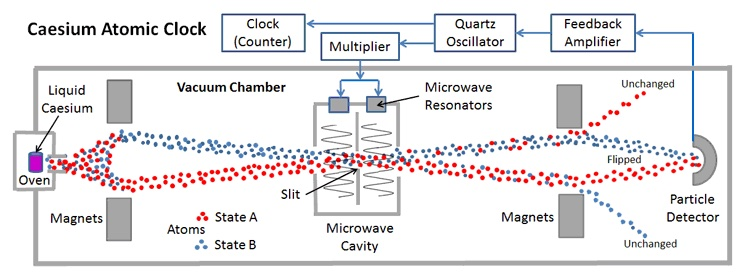
\includegraphics[width=0.85\textwidth]{./Bilder/Atomic_Clock.jpg}
\caption{\label{fig_Atomuhr}%
Prinzip einer C\"asium-Uhr: Aus einem Ofen str\"omen C\"asium-Atome nahezu gleichverteilt im
Grundzustand und im angeregten Hyperfeinstrukturzustand. In einem Magnetfeld werden die
Atome im Grundzustand von denen im angeregten Zustand getrennt (sie haben unterschiedliche
magnetische Momente) und treten dann unter einem unterschiedlichen Winkel in einen
Resonator. In diesem Resonator werden sie einem oszillierenden Feld ausgesetzt, dessen Frequenz
\"uber eine R\"uckkopplung auf die Eigenfrequenz des \"Ubergangs eingestellt wird. Dadurch werden die
Atome zu \"Uberg\"angen angeregt. In einem Detektor hinter dem Resonator wird die Anzahl der Atome
gemessen, die einen \"Ubergang gemacht haben -- je genauer die Resonatorfrequenz auf die
\"Ubergangsfrequenz eingestellt ist, umso mehr Atome werden zu einem \"Ubergang angeregt. Der
Detektor steuert \"uber die R\"uckkopplung die Frequenz des Resonators, sodass m\"oglichst viele
Atome den Detektor erreichen. Abgelesen wird die Frequenz des Resonators. (aus \cite{Atomuhr})}   
\end{figure}

In einem Resonator werden die C\"asiumatome zu \"Uberg\"angen angeregt (Abb.\ \ref{fig_Atomuhr}), wobei
der Anteil der Atome, die einen \"Ubergang machen, umso h\"oher ist, je n\"aher die Frequenz des
Resonatorfeldes an der \"Ubergangsfrequenz liegt. Die Frequenz des Resonatorfeldes wird von einem
Quarzkristall gesteuert, der wiederum von einem Detektor hinter dem Resonator gesteuert wird. 
Dieser Detektor misst die Anzahl der Atome, die einen \"Ubergang gemacht haben, und er steuert den
Quarzkristall so, dass diese Anzahl maximal bleibt. An dem Quarzkristall wird dann auch die jeweilige
Frequenz abgelesen und in eine Uhrzeit umgewandelt. 

Moderne\index{Opticlock} 
Atomuhren arbeiten bei optischen Frequenzen und erreichen damit nochmals eine um
einen Faktor 1000 bis 10\,000 h\"ohere Genauigkeit. Sie befinden sich derzeit in der Testphase,
es wird aber nicht ausgeschlossen, dass in einigen Jahren die Sekunde \"uber solche Opticlocks
neu festgelegt wird. 

\subsection{Fountain-Clocks}

Das bisher beschriebene Verfahren beruht auf Ideen von 
Isidor Isaac Rabi\index{Rabi, Isidor Isaac}\index{Ramsey, Norman} 
Mitte des letzten Jahrhunderts.
Diese Ideen wurden von seinem \glqq Sch\"uler\grqq\ Norman Ramsey nochmals erweitert und zu gr\"o\ss erer
Pr\"azision gef\"uhrt. Eine wesentliche Verbesserung besteht darin, die Cs-Atome zweimal f\"ur einen
kurzen Augenblick durch einen Resonator zu schicken, wobei die Pr\"azession der Uhr umso gr\"o\ss er ist, je
mehr Zeit zwischen diesen beiden Augenblicken liegt.\index{Fountain-Clock} 
In sogenannten Fountain-Clocks (\glqq Springbrunnen-Uhren\grqq)
werden die C\"asiumatome zun\"achst abgek\"uhlt (d.h.\ verlangsamt, dies geschieht mit Laserk\"uhlung) 
und dann mit wenigen Metern pro
Sekunde senkrecht nach oben gesto\ss en. Sie durchlaufen in einem freien Fall eine Parabelkurve, wobei
sie zu Beginn und am Ende kurz durch einen Resonator fliegen. Auf diese Weise befinden sich die C\"asiumatome 
wesentlich l\"anger in der Phase zwischen den Resonatoreinfl\"ussen und die Genauigkeit der Frequenz 
kann besser reguliert werden. 

\section{Kuriosit\"aten}

\subsection{Die tautochrone Kurve -- Zykloide}

Nachdem Galilei erkannt hatte, dass bei einem Pendel die Periode bei kleinen Auslenkungen
nahezu unabh\"angig von der Amplitude des Pendels ist, hatte 
Christiaan Huygens\index{Huygens, Christiaan} 
1656 die Idee, ein Pendel als Taktgeber einer Uhr zu verwenden. Ihm war jedoch
bewusst, dass bei einem realen Pendel die Periode nicht vollkommen unabh\"angig von der Auslenkung
ist und bei gro\ss en Auslenkungen doch deutliche Abh\"angigkeiten von der Amplitude auftreten.
Huygens stellte sich daraufhin die Frage, wie man erreichen kann, dass die Periodendauer eines
Pendels vollkommen unabh\"angig von der Auslenkung ist. 

Das theoretische Problem besteht zun\"achst darin, die Bahnkurve zu bestimmen, die ein
Massenpunkt durchlaufen muss, sodass die Periode der Schwingung unabh\"angig von der Auslenkung ist.
Eine solche Bahnkurve bezeichnet man als\index{tautochron}\index{isochron} 
tautochrone oder auch isochrone Bahnkurve.
Eine Kreiskurve, wie sie bei einem Pendel konstanter Pendell\"ange durchlaufen wird, hat diese 
Eigenschaft nur bis auf Terme 4.\ Ordnung in der Auslenkung (z.B.\ im Auslenkungswinkel) und daher
nur f\"ur kleine Auslenkungen. Das
zweite, eher praktische Problem besteht in der Konstruktion eines Aufh\"angemechanismus,
sodass die Masse an einem Fadenpendel tats\"achlich die tautochrone Bahnkurve durchl\"auft.

Man kann analytisch mit Variationsrechnung die Form dieser Bahnkurve herleiten. Wir geben hier jedoch das 
Ergebnis an und beweisen, dass diese Bahnkurve die gew\"unschten Eigenschaften hat. 
Es handelt sich um\index{Zykloide}
eine sogenannte Zykloide, wie sie in Abb.\ \ref{fig_Zykloide} dargestellt ist. Eine Zykloide wird von einer
Markierung am Rand eines Kreises beschrieben, wenn dieser Kreis an einer Geraden entlang rollt. 

\begin{figure}[htb]
\begin{tikzpicture}
\draw (9.5,2) circle (2.0cm);
\draw (7.28,2) circle (2.0cm);
\draw [->] (0,4) -- (15,4);
\draw (14.7,3.9) node{${\scriptstyle x}$}; 
\draw [->] (7.28,4) -- (7.28,-1);
\draw (7.4,-0.8) node{${\scriptstyle y}$}; 
\draw (9.5,4) -- (9.5,0);
\draw (7.72,2.9) -- (11.28,1.1);
\draw (9.5,4) -- (11.28,1.1);
\draw (9.5,0) -- (13.5,2.46);
\draw (11.28,1.1) -- (13.5,1.1);
\draw (11.28,1.1) -- (9.5,1.1);
\filldraw[fill=red] (1,4) circle(0.08cm);
\draw (1,4.2) node{${\scriptstyle A}$}; 
\filldraw[fill=red] (13.57,4) circle(0.08cm);
\draw (13.57,4.2) node{${\scriptstyle D}$}; 
\filldraw[fill=black] (7.28,4) circle(0.05cm);
\draw (7.28,4.2) node{${\scriptstyle E}$}; 
\filldraw[fill=red] (7.28,0) circle(0.08cm);
\draw (7.4,-0.2) node{${\scriptstyle B}$}; 
\filldraw[fill=red] (11.28,1.1) circle(0.08cm);
\draw (11.35,0.9) node{${\scriptstyle C}$}; 
\filldraw[fill=black] (7.72,2.9) circle(0.05cm);
\draw (7.98,3.0) node{${\scriptstyle E'}$}; 
\filldraw[fill=black] (9.5,2) circle(0.05cm);
\draw (9.28,1.83) node{${\scriptstyle M'}$}; 
\filldraw[fill=black] (7.28,2) circle(0.05cm);
\draw (7.1,2.0) node{${\scriptstyle M}$}; 
\filldraw[fill=black] (9.5,4) circle(0.05cm);
\draw (9.5,4.2) node{${\scriptstyle F}$}; 
\filldraw[fill=black] (9.5,1.1) circle(0.05cm);
\draw (9.3,1.1) node{${\scriptstyle G}$}; 
\draw (13.0,2.0) node{${\scriptstyle t}$}; 
\draw (4.0,4.13) node{${\scriptstyle a}$}; 
\draw (10.4,1.4) node{${\scriptstyle r}$}; 
\draw (7.12,1) node{${\scriptstyle r}$}; 
\draw (11.7,1.23) node{${\scriptstyle \theta}$}; 
\draw[thick] (1,4) .. controls (1,2.9) and (3.17,0) .. (7.28,0); 
\draw[thick] (7.28,0) .. controls (11.4,0) and (13.57,2.9) .. (13.57,4); 
\draw (7.28,4) .. controls (7.28,3.6) and (7.4,3.2) .. (7.72,2.9); 
\draw (9.65,1.8) node{${\scriptstyle \alpha}$}; 
\draw (9.38,2.2) node{${\scriptstyle \alpha}$}; 
\draw (9.6,3.6) node{${\scriptstyle \theta}$}; 
\draw (11.0,1.4) node{${\scriptstyle \theta}$}; 
\draw (9.65,2.12) node{${\scriptstyle \gamma}$}; 
\draw (9.5,1.6) arc (270:515:0.4cm);
\draw (9.5,3.4) arc (270:300:0.6cm);
\draw (10.98,1.58) arc (115:150:0.5cm);
\draw (11.9,1.1) arc (0:30:0.6cm);
\end{tikzpicture}
\caption{\label{fig_Zykloide}%
Die Zykloide. Wenn ein Kreis (Radius $r$) auf einer geraden Linie $a$ (gleichzeitig die $x$-Achse)
abrollt, beschreibt ein Punkt $B$ auf dem
Rand des Kreises (rot eingezeichnet) den Bogen einer Zykloide. Es gilt immer $\alpha=2\theta$, da
sowohl $\alpha + \gamma$ als auch $\gamma + 2\theta$ einem Winkel von $180^\circ$ entsprechen.
Die Tangente $t$ im Punkt $C$ steht senkrecht auf der Verbindungslinie $\overline{FC}$ und schlie\ss t
mit einer Waagerechten einen Winkel $\theta$ ein. Der Nullpunkt des Koordinatensystems sei der
Punkt $E$. Wenn der Kreis in diesem Punkt die Achse $a$ ber\"uhrt, sei $B$ am Minimum der Kurve, also
auf dem Kreis dem Punkt $E$ gegen\"uber.} 
\end{figure}

Wir w\"ahlen den Nullpunkt unseres Koordinatensystems als den Ber\"uhrungspunkt $E$ des Kreises mit der
Geraden an der Stelle, wo die Markierung (Punkt $B$) im Mininum ist. Rollt der Kreis
um einen Winkel $\alpha$ nach rechts, ist der Ber\"uhrungsgpunkt mit der Geraden der Punkt $F$. Die
Distanz zwischen $E$ und $F$ ist genau gleich der Bogenl\"ange zwischem dem ehemaligen Ber\"uhrunsgpunkt
(jetzt $E'$) und dem Punkt $F$, also $\overline{EF}=\alpha r$, wobei der Winkel $\alpha$ in Radianten ausgedr\"uckt
wird. Der Punkt $B$ hat sich bis zum Punkt $C$ weiterbewegt und dabei den
Bogenabschnitt der Zykloide \"uberstrichen.

Wir geben zun\"achst eine Parametrisierung der Zykloide an: Die $x$- und die $y$-Koordinate werden als
Funktion des Winkels $\alpha\in [-\pi,+\pi]$ beschrieben:
\begin{equation}
        x(\alpha) = r ( \alpha + \sin \alpha )    \hspace{1cm} , \hspace{1cm}   y(\alpha) = - r (1+  \cos \alpha ) \, .
\end{equation}
Die $x$-Koordinate ergibt sich aus der Summe von zwei Beitr\"agen: $\overline{EF}+\overline{GC}=r\alpha + r\sin \alpha$,
und die $y$-Koordinate ergibt sich aus: $\overline{FM'} + \overline{M'G}=r + r\cos \alpha$ (in die negative $y$-Richtung). 

Zum Beweis, dass die Zykloide tats\"achlich  die L\"osung des Problems darstellt, ist zu zeigen, dass die
Kraft proportional zur Bogenl\"ange der Auslenkung ist, dass es sich also um einen idealen harmonischen Oszillator
handelt. Dies unterscheidet die Zykloide von einer Parabel: Bei einer Parabel ist die Kraft proportional
zur Auslenkung in $x$-Richtung (oder, was \"aquivalent ist, das Potenzial ist proportional zum Quadrat der 
Auslenkung in $x$-Richtung), bei einer Zykloide ist die Kraft proportional zur Bogenl\"ange. Die Richtung der 
Kraft ist tangential zur Kurve und somit ist 
\begin{equation}
        F=mg \sin \theta=mg \sin \frac{\alpha}{2} \, .
\end{equation} 
Die Bogenl\"ange entlang der Zykloide (also zwischen $B$ und $C$) erhalten wir aus
\begin{eqnarray}
   {\rm d}s^2 &=& \left( \left( \frac{{\rm d} x}{{\rm d}\alpha} \right)^2 + \left( \frac{{\rm d} y}{{\rm d}\alpha} \right)^2 \right) 
                                     ({\rm d}\alpha)^2 \\ 
       &=&  \left( r^2 (1 + \cos \alpha)^2 + r^2 (\sin \alpha)^2 \right) ({\rm d}\alpha )^2 \\
       &=&   2 r^2 ( 1 + \cos \alpha) ({\rm d}\alpha )^2 \, .
\end{eqnarray}
Mit der trigonometrischen Beziehung
\begin{equation}
   1 + \cos \alpha = 1 + \cos^2 \frac{\alpha}{2} - \sin^2 \frac{\alpha}{2} = 2 \cos^2 \frac{\alpha}{2} 
\end{equation}
folgt
\begin{equation}
      {\rm d}s = 2r \cos \left( \frac{\alpha}{2} \right) \,  {\rm d} \alpha 
\end{equation}
und damit
\begin{equation}
      s = 2 r \int_0^\alpha \cos \left( \frac{\alpha'}{2} \right) \,  {\rm d} \alpha' = 
            4r  \left. \sin \frac{\alpha'}{2} \right|_0^\alpha = 4r \sin \frac{\alpha}{2}   \, .
\end{equation}
F\"ur die Zykloide gilt also tats\"achlich, dass die Bogenl\"ange proportional zur r\"ucktreibenden
Kraft ist und damit handelt es sich um einen idealen harmonischen Oszillator mit einer von der
Auslenkung unabh\"angigen Periode. 

\begin{SCfigure}[50][htb]
\begin{tikzpicture}[scale=0.5]
\draw (0,4) -- (14.6,4);
\draw [thick] (7.28,4) -- (7.28,-4);
\fill[gray!20!white]  (1,4) -- (1,0) .. controls (5.12,0) and (7.28,2.9) .. (7.28,4) -- (1,4); 
\fill[gray!20!white]  (7.28,4) .. controls (7.28,2.9) and (10.24,0) .. (13.56,0) -- (13.56,4) -- (7.28,4); 
\draw (1,0) .. controls (5.12,0) and (7.28,2.9) .. (7.28,4); 
\draw [thick] (7.28,4) .. controls (7.28,2.9) and (10.24,0) .. (13.56,0); 
\filldraw[fill=black] (7.28,4) circle(0.05cm);
\filldraw[fill=black] (7.28,-4) circle(0.1cm);
\filldraw[fill=black] (13.56,0) circle(0.1cm);
\draw [thick] (12.42,-2) -- (8.24,2.4);
\draw [thick] (7.28,4) .. controls (7.28,3.7) and (7.4,3.3)  .. (8.24,2.4);
\filldraw[fill=black] (12.42,-2) circle(0.1cm);
%
\draw (1,0) .. controls (1,-1.1) and (3.17,-4) .. (7.28,-4); 
\draw (7.28,-4) .. controls (11.4,-4) and (13.57,-1.1) .. (13.57,0); 
\end{tikzpicture}
\caption{\label{fig_Zykloide2}%
Die Huygens'sche Aufh\"an\-gung. Die Zykloide l\"ost gleichzeitig das zweite Problem bez\"uglich eines
von der Auslenkung unabh\"angigen Pendels: Wenn das schwingende Pendel an seiner Aufh\"angung
durch eine Zykloide begrenzt ist, sodass der obere Teil des Pendelseils an der Zykloide entlang
l\"auft, folgt die Masse am Ende des Pendels einer Zykloide.} 
\end{SCfigure}

Das zweite Problem des Huygens'schen Pendels, die Aufh\"angung, wird ebenfalls durch die Zykloide
gel\"ost.\index{Huygens'sche Pendelaufh\"angung} 
Abbildung \ref{fig_Zykloide2} zeigt, wie man die Aufh\"angung eines Pendels durch eine Zykloide
eingrenzen kann, sodass die Pendelmasse tats\"achlich die Trajektorie einer Zykloide durchl\"auft. 
Dies bezeichnet man auch als die Huygens'sche Pendelaufh\"angung.


Huygens erhoffte sich durch einen solchen Mechanismus
eine tautochrone Schwingung des Pendels auch unter extremen Bedingungen (z.B.\ auf einem
dem Wind und Wellen ausgesetzten Schiff). Letztendlich war diese Idee nicht erfolgreich, statt dessen wurden bessere
Hemmungen, die unter anderem kleinere Auslenkungen erm\"oglichten, entwickelt. 

\begin{thebibliography}{99}

\bibitem{Niermann} 
Till Niermann - Eigenes Werk, CC BY-SA 3.0, \url{https://commons.wikimedia.org/w/index.php?curid=21792620}

\bibitem{Atomuhr} aus: Electropaedia ``Clock and Watch Movements'', 
           \url{https://mpoweruk.com/timekeepers.htm}
\bibitem{Foliot} aus Wikipedia ``Foliot''. \url{https://de.wikipedia.org/wiki/Foliot#/media/Datei:Foliot.jpg}.
\bibitem{Verge} Spindel-Hemmung; \url{https://www.youtube.com/watch?v=UhFPb-ZZTyI}
\bibitem{Neugebauer} O.\ Neugebauer; \textit{A History of Ancient Mathematical Astronomy}, 
       Studies in the History of Mathematics and Physical Sciences 1; Springer-Verlag Berlin
       Heidelberg GmbH, 1975.
\bibitem{Sobel} Dava Sobel; \textit{Longitude}, Fourth Estate, Second Printing 1995. Deutsch: \textit{L\"angengrad};
                  Malik, National Geographic, 2013.        
\end{thebibliography}

%\end{document}

